\documentclass{exam}
\usepackage{mycommands,amsmath,amsfonts,tikz,xeCJK}
\setCJKmainfont{STSong}
\begin{document}
\begin{questions}
    \question
    设$D$是由可求长简单闭曲线$\gamma$围成的域,如果$f\in H(D)\cap C(\bar D)$,那么对任意$z\in D$,均有
  \begin{equation}\label{eq3.4.1}
    f(z) = \frac{1}{2\pi i}\int\limits_\gamma\frac{f(\zeta)}{\zeta-z}\diff \zeta.
  \end{equation}
  \begin{minipage}{0.3\textwidth}
    \centering
    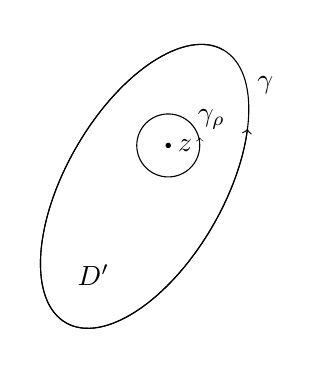
\begin{tikzpicture}
      \draw[rotate=60](0,0)circle(2 and 1);
      \draw[rotate=60,->,thin](2,0)arc(0:310:2 and 1);
      \draw(60:0.6)circle(0.4);
      \fill(60:0.6)circle(1pt)node[right]{$z$};
      \draw(45:1.2)node{$\gamma_\rho$}(40:2)node{$\gamma$}(-120:1.3)node{$D'$};
      \draw[->,very thin]([xshift=0.4cm]60:0.6)--++(0,0.1);
    \end{tikzpicture}
  \end{minipage}
  \newpage
  \question
  设$\gamma$是$\MC$中的可求长曲线,$g$是$\gamma$上的连续函数,定义
  \[
    G(z) = \frac1{2\pi i}\int\limits_\gamma\frac{g(\zeta)}{\zeta-z}\diff \zeta,
  \]
 在$\MC\backslash\gamma$上有任意阶导数,而且
  \begin{equation}\label{eq3.4.4}
    G^{(n)}(z) = \frac{n!}{2\pi i}\int\limits_\gamma \frac{g(\zeta)}{(\zeta-z)^{n+1}}\diff \zeta,n=1,2,\cdots.
  \end{equation}
  \newpage
  \question
  \begin{parts}
  \part
  设$D$是由可求长简单闭曲线$\gamma$围成的域,如果$f\in H(D)\cap C(\bar D)$,那么$f$在$D$上有任意阶导数,而且对任意$z\in D$,有
  \begin{equation*}
    f^{(n)}(z) = \frac{n!}{2\pi i}\int\limits_\gamma\frac{f(\zeta)}{(\zeta-z)^{n+1}}\diff \zeta,n=1,2,\cdots.
  \end{equation*}
  \part
  如果$f$是域$D$上的全纯函数,那么$f$在$D$上有任意阶导数.
  \end{parts}
  \vspace*{3in}
  \question
  计算积分
  \[
    \int\limits_{|z|=2} \frac{\diff z}{(z^3-1)(z+4)^2}.
  \]
  \begin{figure}[!ht]
    \raggedright
    \begin{tikzpicture}[scale=0.5]
      \draw(0,0)node[below]{$O$}--(2,0)node[below right]{$2$}--(5,0)node[right]{$R$};
      \draw(70:2)arc(70:433:2)node[above right]{$\gamma_2$};
      \draw[->](70:5)arc(70:433:5)node[above right]{$\gamma_1$};
      \fill(0,0)circle(2pt)(2,0)circle(2pt)(5,0)circle(2pt);
      \draw[->,very thin](70:2)--++(160:0.1);
    \end{tikzpicture}
  \end{figure}
  \newpage
  \question
  \begin{parts}
    \part
    Cauchy不等式:设$f$在$B(a,R)$中全纯,且对任意$z\in B(a,R)$,有$|f(z)|\le M$,那么
    \begin{equation}\label{eq3.5.1}
        |f^{(n)}(a)|\le\frac{n!M}{R^n}, n=1,2,\cdots.
      \end{equation}
    \part
    有界整函数必为常数.
    \part
    代数学基本定理:任意复系数多项式
    \[
    P(z) = a_0z^n + a_1z^{n-1} + \cdots + a_n,a_0\ne0
    \]
  在$\MC$中必有零点.
  \part
  Morera定理:如果$f$是域$D$上的连续函数,且沿$D$内任一可求长闭曲线的积分为零,那么$f$在$D$上全纯.
  \end{parts}
\end{questions}
\end{document}